% --
% Introduction

\chapter{Introduction}\label{sec:intro}
Controlling video games with the voice of a player in order to render certain actions within the game, is an interdisciplinary challenge between speech signal processing, machine learning and game design.
A microphone is required to capture the voice of a player providing a speech signal of a potential command for the video game.
The speech signal is usually extracted from raw audio samples to meaningful features, such as the Mel Frequency Cepstral Coefficients (MFCC) and being used as inputs to a Key Word Spotting (KWS) system with the task of classifying those features to the most probable command.
The spoken command should change states of specific game objects and therefore ideally enhance and extend the gaming experience of the players.
A simple schematic of the whole process is shown in \rfig{intro_kws}.
\begin{figure}[!ht]
  \centering
    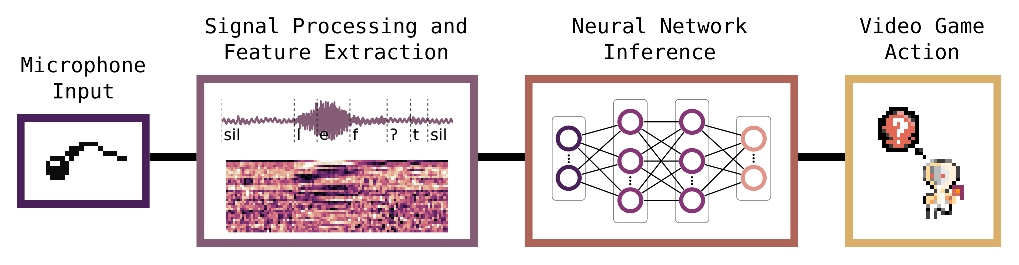
\includegraphics[width=0.9\textwidth]{./1_intro/figs/intro_kws}
  \caption{Simplified process of key word spotting for video games.}
  \label{fig:intro_kws}
\end{figure}
\FloatBarrier
\noindent
In the semantic perspective, the controlling of game objects, should be short, clear and best done with single command words, referred as speech commands.
Single words are easier to detect in comparison to long sentences, for instance it is easier to recognize the word \enquote{left} than the sentence \enquote{missile target on position x, y}.
The classification of those speech commands can be done with a KWS system composed of a neural network.
KWS is restricted by a limited set of selected key words, referred as vocabulary or class dictionary.
In terms of video games, the set of key words might have members like \enquote{left} or \enquote{right}, for instance to move an element within the game to either left or right respectively.
The limited set of key words is crucial to restrict the complexity of the recognition task, since in practical applications it is not necessary to cover all words in a natural language.
Especially in video games, where the game environment is restricted by rules, technical limits and play-ability, KWS is suited perfectly as an alternative or augmented control system.
The size of the vocabulary and the selected words are two parameters that influence on one hand the choice of the neural network architecture, evaluated on energy efficiency and accuracy performance and on the other hand the game experience over the controls a player can choose from.
If the vocabulary of a KWS system would be too large, the chance of confusion between two different key words grows naturally.
In many KWS applications it is absolutely necessary to include labels for \emph{background noise}, \emph{silence} and \emph{unknown words} in the vocabulary. 
This is especially interesting in \emph{wake word} applications, where a single key word must be detected over the previously mentioned labels representing all other possible words that can be spoken.
Also in video games those additional labels are useful to prevent the player from eliciting unintended commands accidentally, through for instance loud background noise.
Therefore a KWS system has the demand of being very accurate and fast in its classification of key words.

Nowadays KWS systems are considered no science-fiction anymore, assisting consumers in everyday situations, such as rendering simple control tasks as the triggering of a photo release button on a \emph{smartphone} with a single speech command.
Application like this create more awareness of KWS, or generally speaking of speech recognition tasks, in human society.
Unfortunately some consumer applications with integrated speech recognition systems, leave a bitter aftertaste in data privacy issues and energy consumption through an externally and extensive computational processing pipeline over corporate servers \cite{Tang2018}.
It is therefore important to create incorporated KWS systems that respect private user data and provide an efficient implementation to save energy consumption.

Video games are a potential application for KWS, until now however, there exist very few of them with this special feature.
Reasons for that might be found in the history of video games itself, where players find themselves in fast paced arcade games and speech recognition was simply too slow.
Additionally the complexity of KWS and lack of training data are often two valid arguments for not considering the deployment of a KWS system in a video game.

The following two sections in this introduction will briefly show the contributions of this thesis and give an overview of upcoming sections.
In summary, the focus of this thesis lies on KWS with neural networks trained through supervised learning on a speech command dataset \cite{Warden2018}.
The best suitable solutions for speech commands classification for video games are presented and evaluated with special interests in Convolutional Neural Networks (CNN), Generative Adversarial Neural Networks (GAN) and Wavenets.

% contributions
% --
% contributions

\section{Contributions}
A KWS system for video games requires fast response times.
Therefore, it is essential to reduce the classification time interval from the examples of the used speech commands dataset \cite{Warden2018SpeechCommands} from \SI{1}{\second} to at most \SI{500}{\milli\second}.
This can be achieved by determining the onset of the highest energy region within the speech signal by extracting the MFCCs and using the first cepstral coefficient as energy measure.
From the determined onset, the desired time interval is cut out of the original data example and used for further processing.

CNN models with low computational footprints, such as examined in \cite{Sainath2015KWS}, are the main evaluation subject within this thesis.
Besides a low computational footprint of the CNN models, the aim is to minimize the amount of neural network layers in order to reduce the complexity of the internal model structure.
The use of MFCC features as inputs to the CNN models required the conduction of experiments upon the number of cepstral coefficients and possible enhancements of MFCCs, such as delta, double delta, and energy features.
It is explained why a reduction of cepstral coefficients and sparing of enhancements are often preferred, especially for a computationally efficient solution.

A frame-based normalization (normalization regarding the time dimension) is introduced and performed on MFCCs to suite them better for visualization and GAN training.
Evaluation of the frame-based normalization is done in terms of recognition accuracy, and shift and noise invariance on conventional CNN models.
Moreover, the advantages and disadvantages of such a normalization technique are discussed.

Another large evaluation topic within this thesis is the application of GANs to generate new examples from the speech command dataset.
Note that GANs consist of a Generator (G) and Discriminator (D) network that are trained to compete against each other.
By applying frame-based normalization to the MFCC extracted speech command examples with the purpose to limit their values in the range of $[0, 1]$, G learns faster to produce fake images.
In the experiments it was found that when G and D were trained for too long, a noisy equilibrium state may emerge, where both networks generate random outputs of either fake images or decisions.
To solve this problem, a second loss term for G was added that measures the similarity of the generated samples to the input data by applying the cosine distance.
This helped to improve the generation of fake images and did not lead into noisy equilibrium states anymore.

Moreover, from the adversarial training of GANs, it is examined how the obtained weights can contribute to the performance of an equivalent CNN model with the same convolutional layer structures.
The transfer of the obtained weights (transfer learning) from either D or G is used in order to initialize the target CNN model for the KWS task.
The experiments show that the obtained weights of G can be very valuable when frame-based normalization is applied.

A completely different approach to the KWS task was the evaluation of a Wavenet \cite{Oord2016Wavenet} model for classification.
However, the initial assumption that without feature extraction a lower amount of computations is required in the application of an online system for video games, finally turned out to be wrong.
Wavenets have to run a huge amount of operations by processing each sample of the audio files from the dataset through dilated convolutional filters over many layers.
Furthermore, the classification accuracy of a reasonable sized Wavenet turned out to be very poor compared to the CNN approaches.
Nevertheless, this model with an extension for class predictions was evaluated and the obtained results are reported.

The integration of the KWS system into the video game is explained, where the KWS system consists of an online system for capturing the microphone input stream and a classification system that maps speech commands to certain actions within the game.

% overview
% --
% intro overview of thesis

\section{Overview}\label{sec:intro_overview}
After this introduction, \rsec{back} provides background information of the individual disciplines within this thesis, further some research questions are listed and give insight into problems of the KWS task for video games.
\rsec{prev} lists previous and related work, where a small history about neural networks is given and important works on neural network architectures are referenced, as well as works that influenced and motivated this thesis.
The audio signal processing part is located in \rsec{signal} and explains the extraction of meaningful features for speech recognition, such as MFCCs and an onset detection method for KWS.
The feature extraction and onset detection is guided with examples to visualize their properties.
In \rsec{nn} theory about neural networks in general, as well as the used neural networks architectures and the adversarial pre-training are described.
The experiments are presented in \rsec{exp} with a thorough observation of the dataset and a general listing of experimental details beforehand. 
Experiments were conducted on the feature selection of MFCCs, the adversarial pre-training, the Wavenet architecture and the final experiments running on the whole dataset.
\rsec{game} describes the integrated KWS system in detail and presents the game design of the deployed video game.
The thesis finishes with a conclusion and an outlook to future work in \rsec{conclusion}.


% --
% background section

\chapter{Background}\label{sec:back}
This section provides fundamental background information regarding KWS, neural networks and video games.
The KWS task is described mathematically to express the actual speech recognition problem.
Notes on neural networks explain common properties and terms in their application.
Research questions are listed and give a deeper insight in common challenges of implementing a KWS system into a video game.

% disciplines
% --
% Intro of keyword spotting

\section{The Keyword Spotting Task}\label{sec:intro_kws}
As described in \rsec{intro}, KWS is the task of classifying speech signals of spoken words to single keywords out of a set of keywords.
The set of keywords $S$, also referred to as vocabulary, can be defined by
\begin{equation}\label{eq:intro_kws_dict}
	S \coloneqq \{s_i \mid i = 0, 1, \dots, L\},
\end{equation}
where $s_i$ represents the $i$-th keyword of a set of $L$ keywords.
The task is to select the keyword closest to the spoken word from the user, denoted as target $t$.
The target does not necessarily have to be a member of the set of keywords $S$, in fact it can be any arbitrary word.
With the abstract formulation
\begin{equation}\label{eq:intro_kws_task}
	\hat{s} = \underset{s_i \in S}{\arg \min} \, \mathcal{D}(t, s_i),
\end{equation}
the most probable keyword $\hat{s}$ can be predicted, where $\mathcal{D}$ is some kind of distance measure between two words.
The formulation in \req{intro_kws_task} is merely semantic but KWS in computer systems have to cope with various transformations of raw input samples $\bm{x} \in \R^n$ of audio data with a total number of $n$ samples.
An inference from audio data to output class probabilities $\bm{y} \in \R^L$ can, for example, be achieved by the use of a neural network containing a softmax function at its last layer (transforming the output of the last layer to probability values).
The most probable keyword can therefore be picked by
\begin{equation}\label{eq:intro_kws_class}
	\hat{s} = \{s_i \mid \underset{i = 0, 1, \dots, L}{\arg \max} \, y_i\},
\end{equation}
where the index $i$ of the output class probability $y_i$ corresponds to the intended keyword $s_i$ in the vocabulary.

In comparison to full Automatic Speech Recognition (ASR), where whole sentences need to be identified, KWS operates merely on the word level.
Therefore, KWS is slightly easier to deploy and less complex than ASR.
Conversely, KWS systems have to run very energy efficiently on low-resource devices, such as mobile phones, and provide immediate and accurate responses to the users.
A good elaboration on the requirements of KWS systems can be found in the motivation section of \cite{Warden2018}.
% --
% Intro to neural networks

\section{Notes on Neural Networks}\label{sec:intro_nn}
Neural networks enable computers to automatically learn from data to be able to solve tasks, such as pattern recognition in images or audio.
The \emph{training} of a neural network with a specific dataset, is the learning process of all parameters within its architecture.
The examples or samples from the input data can be paired with annotations, denoted as \emph{labels} or \emph{classes}.
If the label information of each example is used during the training of a machine learning system, such as a neural network, it is called \emph{supervised learning} otherwise it is called \emph{unsupervised learning}.
Yet supervised learning is more commonly applied.
\emph{Inference} is simply the forward pass of input data samples through an already trained network to output their estimated class labels.

The main advantage of neural networks is that they are able to cope with large amounts of input variables per data example.
Considering a raw waveform file of merely \SI{1}{s} time duration, sampled with \SI{16}{\kilo\hertz} would give an input size of 16000 features.
This huge amount of input features is even difficult for neural networks to learn from with restricted computational resources and usually a feature extraction stage is placed in between to reduce the input dimension.
For instance, the computation of MFCCs with 12 coefficients and a time duration of \SI{0.5}{s} with a time shift of \SI{10}{\milli\second} reduces the input feature size dramatically to $12 \times 50 = 600$, which is still a high number of input features but much more affordable and faster to train.

Neural networks are able to learn own feature representations, selection and interpretation, rather than using hand-crafted ones done by humans with expertise in the research field.
Note that hand-crafting features of complex recognition tasks is in most cases not even possible or extremely cumbersome.
So researchers prefer neural networks because of their easy deployment scheme and state of the art performances.
Furthermore, it enables everyone capable of using neural network tools to create solutions to rather complex problems, given there is enough data and processing power available.
This causes that elaborate feature extraction stages become less relevant to the users, which may lead to some extend into the ignorance of the classification problem and more \enquote{try and error} approaches of different neural network architectures and training parameters.

The energy consumption required to train Deep Neural Networks (DNN) with many parameters on a huge training dataset, shall not be forgotten, especially in times of climatic change.
Reusing pre-trained weights from renowned network architectures is a good manner to reduce energy consumption in finding an optimal classifier for an already widely examined classification task.
The re-usability of pre-trained weights is often named as \emph{transfer learning}, where a small comprehension on it can be found in \cite{TransferLearning}.

Nevertheless, the potential of neural networks in research are vast.
The observation on how the learning from data is done and what recognition patterns are obtained after training, might allow researchers and experts to better understand the problem or gain a different viewpoint on it.
Especially the use of CNNs allows researchers to visualize the learned filters and interpret their results.
A very interesting example of investigating learned CNN filters is shown by Zeiler et al. \cite{Zeiler2013}.
Other exciting subjects in research are generative models, such as GANs \cite{Goodfellow2014}, which are able to create convincing samples from the learned data distribution.

Neural network architectures for speech recognition are a little bit different from image recognition, mainly because of the sequential nature of time signals.
However, if time signals are restricted in time, which implies that they are limited to a fixed number of samples, and frequency features are extracted over that time span, then speech signals can be represented in 2D space (frequency and time) and classified like images.
That suggests that CNNs are reasonable network architectures for speech as well.
Another potential architecture for audio signals is the Wavenet \cite{Oord2016} because of its ability to process raw audio data.
% --
% video games with speech commands

\section{Video Games with Key Word Spotting}\label{sec:intro_games}
Video games with KWS or any speech input are rarely seen gems in the gaming industry, though it is an exciting and immersive way to interact.
Technically the voice of the player has to be recorded by a microphone, therefore one additional requirement to play the video game is to own a microphone, which however does not need to be high-end.
The input stream of a microphone can be processed through an online or real-time system to extract the input features for the classification system.
The classification system, such as a neural network, is supposed to infer the input information to the intended action within the game.

The processing scheme is easy to define, but not that easy to implement compared to other more hardware based input channels, such as pressing buttons on a keyboard.
Also speech input is very slow compared to hardware input, where players are able to interact within tens of milliseconds (the input lag of gaming controllers should ideally be under \SI{50}{\milli\second}).
This fast response time is not possible with speech, where the player has to physically form a waveform representing the action in the game.
Further the waveform captured from the online system has to be pre-processed, feature extracted and classified to the best estimation of all the available key words in the game's vocabulary.
Concluding this, a good estimate to create and process a speech input should ideally be under one second, the less the better for the playing experience.

Another important consideration has to be made upon the size of the vocabulary.
A high number of key words will increase the chance of confusion and a small number of key words restrict the possible actions a player can choose from.
The possibility to create separate classifiers with different sets of smaller vocabularies of speech commands arises, depending on which commands the player needs in the actual scene of the video game.
For instance, if the player is in a dialogue with a Non Player Character (NPC), it makes sense to reduce the vocabulary to only \{\enquote{yes}, \enquote{no}\}, if those are the only actions to choose from.

The use of labels for background noise, silence and unknown words depends on the game and how the classification process is activated.
If the assumption is made that a player chooses only from the key words in the dictionary, then the label of unknown words is not necessarily required.
However the unknown label would be very interesting if key words are not that common to a player, such as words from a different language or fantasy words.
The unknown label will therefore motivate the player to correctly pronounce the word itself, which could be also used in language learning games.
The labels for background noise and silence are useful in the case of initializing the classification process by the energy value of the input stream of the microphone.
A small impact on the microphone or loud background sound can therefore elicit an unwanted command within the game, if those labels do not exist in the vocabulary.

In KWS video games, players have to act with their voice, which is in some situations not appropriate or annoying, for instance playing a video game in a public transport and shouting into ones mobile phone or laptop might anger other passengers.
Also the slowness of KWS and many other reasons makes it not suitable for every game type.
Luckily the existing types and genres in video games are vast and there might be one or two game ideas where KWS makes a game outstanding, creative and refreshing.
Potential of KWS lies without doubt in the domain of Virtual Reality (VR) and Augmented Reality (AR) applications and games.
In VR the player wears a Head Mounted Device (HMD), where most recent consumer devices have already incorporated a microphone, most commonly used for online chat, but also ready to adopt for KWS.
To increase immersion in VR even further, a KWS systems can be very valuable.

% research questions
% --
% research questions

\section{Research Questions for this Thesis}\label{sec:intro_rq}
This section formulates relevant research questions regarding KWS in video games.
Those research questions can be split into 3 parts:
\begin{enumerate}[label={Q.\arabic*)}, leftmargin=1.4cm]
  \item Signal processing and feature extraction of speech signals.
  \item Neural network training and classification for KWS.
  \item Video games with KWS.
\end{enumerate}
Note that the terms \enquote{key word} and \enquote{speech command} are often named interchangeably because speech commands are used as key words in the KWS system.
Not all research questions can be answered within the scope of this thesis.
Nevertheless, those questions can be asked and some solution concepts discussed.


% --
% signal

\subsection{Signal Processing and Feature Extraction Research Questions}\label{sec:intro_rq_signal}
Acquiring meaningful features from speech signals is essential for neural networks to operate on. 
The features are extracted from raw audio samples of a microphone input stream in a specific time interval.
Those retrieved features are further input to a neural network for the classification of speech commands.
The following Questions arise here:
\begin{enumerate}[label={Q.1.\alph*)}, leftmargin=1.75cm]
  \item Which time interval should be captured to represent a speech command?\label{it:q1-a}
  \item Does the signal processing have to be invariant to background noise and especially to game sounds?\label{it:q1-b}
  \item What are meaningful features for speech recognition?\label{it:q1-c}
\end{enumerate}
\noindent
\textbf{Question \ref{it:q1-a}:} 
The time required to fully pronounce a speech command is not fixed and varies from speaker to speaker, depending also on the intended prolongation a speaker adds to the word.
In practical applications however, a fixed time interval for a single speech command is convenient.
By restricting the time duration of the key words, the speaker has to pronounce the words within this time span.
For example, if a speaker pronounces the word \enquote{left} and requires a time duration of \SI{1}{\second}, hardly all is captured if the time interval is restricted to merely \SI{500}{\milli\second}.
Whether this \SI{500}{\milli\second} is sufficient for a correct classification, is subject for evaluation.
In the application of a video game, the user should preferably speak the commands with a short time duration, so that the game can respond fast.
Problems might occur if the speech commands are spoken repeatedly and very hasty, so that the time interval of consecutive commands overlap each other.
Ideally the time interval to represent a speech command would be flexible but this more difficult to implement than a fixed time interval.

\textbf{Question \ref{it:q1-b}:}
Usually the presence of low background noise should not be a problem for neural networks trained on a large enough data set. 
The game sounds might present a more difficult problem, when turned up too loud without the use of headphones. 
Therefore, the microphone will not only capture the voice of a speaker but also a fair amount of game sounds. 
This problem seems to be theoretically solvable as the shape of the nuisance is known and the amount of game sound in the audio stream could be attenuated sufficiently.
In practice this might be hard to solve without critically disturbing the signal of interest.
A solution to this problem would probably take too much time and effort and is therefore not evaluated within this thesis. 
However, playing a video game without game sound is unsatisfying and it would be a great contribution to tackle this problem in future work.

\textbf{Question \ref{it:q1-c}:} 
The determination of meaningful features for speech signals is a classical problem in speech recognition.
The essential composition of a word may help to understand the problematic better.
A word is a sequential combination of either vowels, such as \enquote{a} and \enquote{e}, or consonants \enquote{k}, \enquote{l}, with a certain length. 
In linguistics for instance, it is possible to distinguish vowels with frequency peaks in a spectrogram, where a spectrogram is the magnitude squared of the frequency response of small time chunks over the time duration of a signal.
However, due to many different factors in voice generation involved in speakers, such as age, gender, nationality and physiology of the vocal tract, there is a huge variance in the pronunciation of words from different persons, which increases the difficulty of the problem.
A very common approach is to use MFCCs as features for speech recognition tasks.
Why MFCCs present good features for speech is described in detail in \rsec{signal_mfcc}.


% --
% neural networks

\subsection{Neural Network Implementation Research Questions}\label{sec:intro_rq_nn}
Neural networks for video games should ideally be very efficient and provide accurate classifications of input features.
The vocabulary in a KWS task has to be specified for the individual game and chosen from all class labels available in the dataset.
Each key word of the vocabulary is presented by one output node of the neural network architecture.
Following Questions can be asked in general:
\begin{enumerate}[label={Q.2.\alph*)}, leftmargin=1.75cm]
  \item Is there an appropriate dataset suited for KWS video games and with sufficient diversity available?\label{it:q2-a}
  \item What happens if an input feature represents a spoken word, which is not in the vocabulary (unknown key word) and how should this exception be handled?\label{it:q2-b}
  \item What is the best neural network architecture regarding classification accuracy and energy efficiency?\label{it:q2-c}
  \begin{enumerate}[label=(\roman*)]
    \item Can adversarial networks improve generalization?
    \item Are Wavenets a solution to this task?
  \end{enumerate}
\end{enumerate}
\noindent
\textbf{Question \ref{it:q2-a}:} 
The availability of a dataset for KWS video games can be answered right away, as there exists a speech commands dataset \cite{Warden2018} with enough and diverse data.
The dataset consist of 35 labels and contains commands for movement and numbers.
Further, it includes randomly selected words like \enquote{marvin} or \enquote{bird} intended to represent \emph{unknown} words for the KWS system.
It has to be noted that not every game idea can be realized with a restricted vocabulary.
Nevertheless, with commands for movement like \enquote{left} or \enquote{go} it is possible to move objects within a game and this can already be used for many game mechanics.
An aspect regarding efficiency, is to restrict the amount of key words in the vocabulary as much as possible such that a cheaper neural network architecture can be deployed, which of course should still be sufficiently good in its classification accuracy.

\textbf{Question \ref{it:q2-b}:} 
Without doubt, players will try out words that are not in the vocabulary (denoted as \emph{unknown} key words) and observe the response of the video game.
The ideal response would be to shown an indication to the player that the word is not present in the vocabulary. 
Nevertheless, it might happen that the similarity of a unknown key word is too close to a key word and an unintended action is triggered in the game. 
At the same time the neural network should not classify key words as unknown key words to ensure a satisfying game experience.
It is better to rely on that players are using key words for most of the time so that they are preferred over unknown key words.

\textbf{Question \ref{it:q2-c}:}
In the ideal case, video games with KWS do not slow down during the inference process of unknown input data.
The restriction of the amount of computations and time for the classification of key words is given by the minimum Frames Per Second (FPS) a video game is perceived as fluent.
That requires the FPS to not fall under a certain limit (usually 30 FPS in video games), otherwise the fluidity of the game is not guaranteed.
Several different neural network approaches with a low computational footprint must therefore be tested and compared against each other regarding classification rate and energy efficiency.
The transfer of weights from GANs is an interesting approach to evaluate whether the trained parameters are also useful for pure classification tasks in CNNs.
Wavenets have the advantage that they do not need a feature extraction stage but it is questionable whether the network design achieves a reasonable computational footprint.


% --
% video games

\subsection{Video Games with KWS Research Questions}\label{sec:intro_rq_games}
Video games that use KWS can create a unique playing experience but must face certain challenges.
Following questions can be stated:
\begin{enumerate}[label={Q.3.\alph*)}, leftmargin=1.75cm]
  \item How should the onset of a key word be detected, so to reduce computations?\label{it:q3-a}
  \item What is the added value of KWS in the gaming experience of players?\label{it:q3-b}
  \item What do game developers have to consider, when designing a game with KWS?\label{it:q3-c}
\end{enumerate}
\noindent
\textbf{Question \ref{it:q3-a}:} 
It is crucial to reduce computations in a video game in order to keep it running fluently during high performance peaks.
Also the unnecessary processing of meaningless input data should be avoided as much as possible.
Ideally the key word classification is activated, when there is actually a speech command present, which however is not always trivial.
One possibility to indicate the onset of a key word is to perform the relatively efficient calculation of an energy value within a certain time interval of the raw input data stream and have a simple threshold value decide, whether a speech command is available. 
To avoid the consecutive triggering of onsets at each energy measure, the microphone and amplifier noise floor and the background sound (including the game sound) have to be less energy intensive than the speech signal obtained from the player.
Another approach similar to the push and talk principle, would be to indicate the onset of a key word with the click of a certain button on the keyboard.
The player is therefore able to control the exact onset of a key word and its length but requires an additional hardware based input channel.

\textbf{Question \ref{it:q3-b}:}
In certain video game scenarios, speech commands can be useful, interesting and enhancing for the gaming experience, in others they might even disturb the game play or even spoil it completely.
It cannot be generally stated whether it is worth to deploy a KWS system into a game, this depends on the game it is intended for.
As already noted in \rsec{intro_games}, KWS might be a great augmented control system for special kind of games to increase the immersion experience, especially for VR applications.
Also language learning games are an interesting application but usually require a huge vocabulary and therefore a phoneme based ASR system would be the better choice.

\textbf{Question \ref{it:q3-c}:}
Apart from the technical requirements involved in KWS systems, also the general game design with KWS has to be considered.
It certainly can be stated that KWS systems are not always reliable and therefore a main game mechanic solely based on it is not always preferred.
Furthermore, the time lag required to process speech commands to actual actions within the game should not be ignored.
The player should for one get immediate and accurate feedback from the game and on the other hand be challenged while playing so that the game experience does not get frustrating or tiresome.
Using speech commands consecutively, can also be very exhausting for the player and maybe it is better to use KWS only in special situations within the game.
Generally it can be stated that a game developer has to design a KWS game with care.